% Options for packages loaded elsewhere
\PassOptionsToPackage{unicode}{hyperref}
\PassOptionsToPackage{hyphens}{url}
\PassOptionsToPackage{dvipsnames,svgnames,x11names}{xcolor}
%
\documentclass[
  xelatex,
  ja=standard]{bxjsarticle}

\usepackage{amsmath,amssymb}
\usepackage{iftex}
\ifPDFTeX
  \usepackage[T1]{fontenc}
  \usepackage[utf8]{inputenc}
  \usepackage{textcomp} % provide euro and other symbols
\else % if luatex or xetex
  \usepackage{unicode-math}
  \defaultfontfeatures{Scale=MatchLowercase}
  \defaultfontfeatures[\rmfamily]{Ligatures=TeX,Scale=1}
\fi
\usepackage{lmodern}
\ifPDFTeX\else  
    % xetex/luatex font selection
  \setmainfont[BoldFont=Noto Sans CJK JP]{Noto Serif CJK JP}
\fi
% Use upquote if available, for straight quotes in verbatim environments
\IfFileExists{upquote.sty}{\usepackage{upquote}}{}
\IfFileExists{microtype.sty}{% use microtype if available
  \usepackage[]{microtype}
  \UseMicrotypeSet[protrusion]{basicmath} % disable protrusion for tt fonts
}{}
\makeatletter
\@ifundefined{KOMAClassName}{% if non-KOMA class
  \IfFileExists{parskip.sty}{%
    \usepackage{parskip}
  }{% else
    \setlength{\parindent}{0pt}
    \setlength{\parskip}{6pt plus 2pt minus 1pt}}
}{% if KOMA class
  \KOMAoptions{parskip=half}}
\makeatother
\usepackage{xcolor}
\setlength{\emergencystretch}{3em} % prevent overfull lines
\setcounter{secnumdepth}{5}
% Make \paragraph and \subparagraph free-standing
\ifx\paragraph\undefined\else
  \let\oldparagraph\paragraph
  \renewcommand{\paragraph}[1]{\oldparagraph{#1}\mbox{}}
\fi
\ifx\subparagraph\undefined\else
  \let\oldsubparagraph\subparagraph
  \renewcommand{\subparagraph}[1]{\oldsubparagraph{#1}\mbox{}}
\fi


\providecommand{\tightlist}{%
  \setlength{\itemsep}{0pt}\setlength{\parskip}{0pt}}\usepackage{longtable,booktabs,array}
\usepackage{calc} % for calculating minipage widths
% Correct order of tables after \paragraph or \subparagraph
\usepackage{etoolbox}
\makeatletter
\patchcmd\longtable{\par}{\if@noskipsec\mbox{}\fi\par}{}{}
\makeatother
% Allow footnotes in longtable head/foot
\IfFileExists{footnotehyper.sty}{\usepackage{footnotehyper}}{\usepackage{footnote}}
\makesavenoteenv{longtable}
\usepackage{graphicx}
\makeatletter
\def\maxwidth{\ifdim\Gin@nat@width>\linewidth\linewidth\else\Gin@nat@width\fi}
\def\maxheight{\ifdim\Gin@nat@height>\textheight\textheight\else\Gin@nat@height\fi}
\makeatother
% Scale images if necessary, so that they will not overflow the page
% margins by default, and it is still possible to overwrite the defaults
% using explicit options in \includegraphics[width, height, ...]{}
\setkeys{Gin}{width=\maxwidth,height=\maxheight,keepaspectratio}
% Set default figure placement to htbp
\makeatletter
\def\fps@figure{htbp}
\makeatother

\renewcommand{\thefootnote}{\arabic{footnote}}
\makeatletter
\makeatother
\makeatletter
\makeatother
\makeatletter
\@ifpackageloaded{caption}{}{\usepackage{caption}}
\AtBeginDocument{%
\ifdefined\contentsname
  \renewcommand*\contentsname{目次}
\else
  \newcommand\contentsname{目次}
\fi
\ifdefined\listfigurename
  \renewcommand*\listfigurename{図一覧}
\else
  \newcommand\listfigurename{図一覧}
\fi
\ifdefined\listtablename
  \renewcommand*\listtablename{表一覧}
\else
  \newcommand\listtablename{表一覧}
\fi
\ifdefined\figurename
  \renewcommand*\figurename{図}
\else
  \newcommand\figurename{図}
\fi
\ifdefined\tablename
  \renewcommand*\tablename{表}
\else
  \newcommand\tablename{表}
\fi
}
\@ifpackageloaded{float}{}{\usepackage{float}}
\floatstyle{ruled}
\@ifundefined{c@chapter}{\newfloat{codelisting}{h}{lop}}{\newfloat{codelisting}{h}{lop}[chapter]}
\floatname{codelisting}{コード}
\newcommand*\listoflistings{\listof{codelisting}{コード一覧}}
\makeatother
\makeatletter
\@ifpackageloaded{caption}{}{\usepackage{caption}}
\@ifpackageloaded{subcaption}{}{\usepackage{subcaption}}
\makeatother
\makeatletter
\@ifpackageloaded{tcolorbox}{}{\usepackage[skins,breakable]{tcolorbox}}
\makeatother
\makeatletter
\@ifundefined{shadecolor}{\definecolor{shadecolor}{rgb}{.97, .97, .97}}
\makeatother
\makeatletter
\makeatother
\makeatletter
\makeatother
\ifLuaTeX
\usepackage[bidi=basic]{babel}
\else
\usepackage[bidi=default]{babel}
\fi
\babelprovide[main,import]{japanese}
% get rid of language-specific shorthands (see #6817):
\let\LanguageShortHands\languageshorthands
\def\languageshorthands#1{}
\ifLuaTeX
  \usepackage{selnolig}  % disable illegal ligatures
\fi
\usepackage[]{natbib}
\bibliographystyle{jecon}
\IfFileExists{bookmark.sty}{\usepackage{bookmark}}{\usepackage{hyperref}}
\IfFileExists{xurl.sty}{\usepackage{xurl}}{} % add URL line breaks if available
\urlstyle{same} % disable monospaced font for URLs
\hypersetup{
  pdftitle={国際社会の成り立ち},
  pdfauthor={土井翔平},
  pdflang={ja},
  colorlinks=true,
  linkcolor={NavyBlue},
  filecolor={Maroon},
  citecolor={NavyBlue},
  urlcolor={NavyBlue},
  pdfcreator={LaTeX via pandoc}}

\title{国際社会の成り立ち}
\usepackage{etoolbox}
\makeatletter
\providecommand{\subtitle}[1]{% add subtitle to \maketitle
  \apptocmd{\@title}{\par {\large #1 \par}}{}{}
}
\makeatother
\subtitle{国際公共政策学}
\author{土井翔平}
\date{2023-05-23}

\begin{document}
\maketitle
\ifdefined\Shaded\renewenvironment{Shaded}{\begin{tcolorbox}[enhanced, borderline west={3pt}{0pt}{shadecolor}, frame hidden, sharp corners, interior hidden, boxrule=0pt, breakable]}{\end{tcolorbox}}\fi

\hypertarget{ux306fux3058ux3081ux306b}{%
\section*{はじめに}\label{ux306fux3058ux3081ux306b}}
\addcontentsline{toc}{section}{はじめに}

現代に国際関係が展開される場としての国際社会が、そのような社会へと至る展開を学ぶ。

\begin{itemize}
\tightlist
\item
  なぜ国家は誕生したのか?
\item
  なぜ主権国家体系が誕生したのか?
\item
  国際社会はどのように展開してきたのか?
\end{itemize}

\hypertarget{ux8ab2ux984cux6587ux732e}{%
\subsection*{課題文献}\label{ux8ab2ux984cux6587ux732e}}
\addcontentsline{toc}{subsection}{課題文献}

\begin{itemize}
\tightlist
\item
  国家

  \begin{itemize}
  \tightlist
  \item
    \citet[第2章]{sunahara2020}
  \item
    \citet[第2章]{kubo2016}
  \item
    \citet[第1章]{kasuya2014}
  \end{itemize}
\item
  国際関係史

  \begin{itemize}
  \tightlist
  \item
    \citet[第1章 (unit 1-5)]{murata2023}
  \item
    \citet[第2章]{nakanishi2013}
  \item
    \citet{ogawa2018}
  \item
    \citet[第1-4章]{yamakage2012}
  \end{itemize}
\end{itemize}

\hypertarget{ux8fd1ux4ee3ux56fdux969bux793eux4f1aux306eux6210ux7acb}{%
\section{近代国際社会の成立}\label{ux8fd1ux4ee3ux56fdux969bux793eux4f1aux306eux6210ux7acb}}

主権国家体系=国家+アナーキーな国際社会はどのようにして生まれたのか?

\begin{itemize}
\tightlist
\item
  人類が誕生したときから国家や主権国家体系が存在していたわけではない。
\item
  人類の選択としての主権国家体系(なぜ?)
\end{itemize}

\hypertarget{ux91cdux5546ux4e3bux7fa9ux6642ux4ee3}{%
\subsection{重商主義時代}\label{ux91cdux5546ux4e3bux7fa9ux6642ux4ee3}}

\begin{figure}[htpb]

{\centering 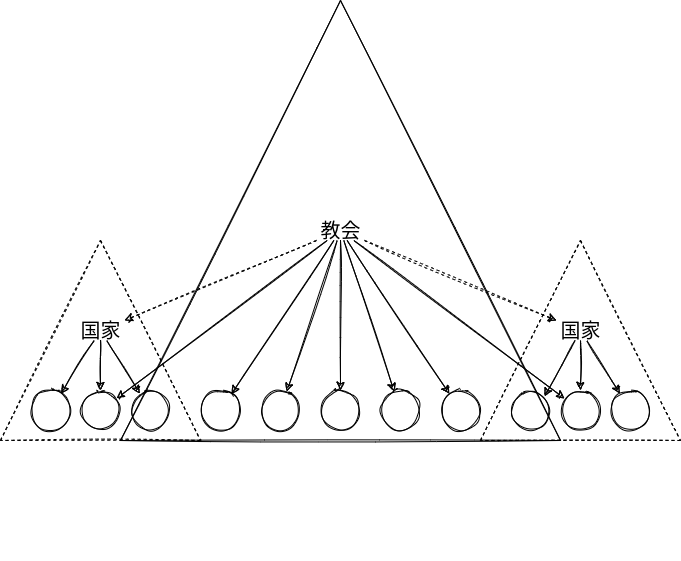
\includegraphics[width=0.8\textwidth,height=\textheight]{figures/hierarchy.drawio.png}

}

\caption{アナーキーではない国際社会のイメージ}

\end{figure}

近世(15世紀後半〜18世紀前半)の西ヨーロッパ:キリスト教権威(ローマ教皇)と政治権力(王国)が混在

\begin{itemize}
\tightlist
\item
  政治権力はキリスト教権威の影響下\(\leadsto\)not主権国家
\item
  領域主権の概念も明確ではなく、キリスト教権威と政治権力が重複することもあった。
\end{itemize}

\(\leadsto\)notアナーキー、but階層 (hierarchy) 的な社会

15世紀半ばからの\textbf{大航海時代}:異なる地域(大陸)同士の交流

\begin{itemize}
\tightlist
\item
  国際社会の誕生、グローバル化の始まり
\end{itemize}

ヨーロッパ諸国:\textbf{重商主義} (mercantilism)
\(\leadsto\)ヨーロッパ外へと進出・植民地の建設

\begin{itemize}
\tightlist
\item
  重商主義:経済的富=軍事力の源泉、軍事力=経済的富の獲得手段
\item
  ヨーロッパ外の市場へのアクセスの確保\(\leadsto\)自らの政治的・軍事的影響力の維持・拡大
\item
  貿易の制限\(\leadsto\)富の流出を回避
\end{itemize}

ヨーロッパ外の地域が植民地となる\(\leadsto\)ヨーロッパの列強諸国間での戦争も勃発

16世紀初めに宗教改革\(\leadsto\)カトリック教会とプロテスタントの対立

\begin{itemize}
\tightlist
\item
  政治権力はプロテスタントをカトリック教会の影響力を排除するために利用
\item
  同時に、自身の宗派の影響力拡大\(\leadsto\)宗教戦争
\end{itemize}

\(\leadsto\)教会権威の低下&国家権力の強化

\hypertarget{ux56fdux5bb6ux306eux8a95ux751f}{%
\subsection{国家の誕生}\label{ux56fdux5bb6ux306eux8a95ux751f}}

\hypertarget{ux6226ux4e89ux3068ux56fdux5bb6}{%
\subsubsection{戦争と国家}\label{ux6226ux4e89ux3068ux56fdux5bb6}}

宗教革命と戦争を通じて、国王に権力(徴税権と暴力)が集中(cf.~官僚制と常備軍)

\begin{itemize}
\tightlist
\item
  銃器の発展\(\leadsto\)大規模な歩兵集団や要塞が必要\(\leadsto\)財政が重要
\item
  財政=軍事国家:軍事のために租税や国債を通じて資金を効率的に集め、返済できる国家が発展・生き残った\citep{brewer2003}。
\item
  「戦争が近代国家を作り、また近代国家が戦争を行う」\citep{tilly1992}
\end{itemize}

国家は国民を外敵から保護すると同時に、税金の見返りとして国民の権利を保障する。

\begin{itemize}
\tightlist
\item
  「マフィアのような犯罪組織と国家との違いは程度問題であって、本質的な違いはない」\citep{tilly1985}
\item
  国家が生き残りのために国力を増強\(\leadsto\)国民の福祉や自由が保障されるかもしれない。
\end{itemize}

\hypertarget{ux5e02ux5834ux3068ux56fdux5bb6}{%
\subsubsection{市場と国家}\label{ux5e02ux5834ux3068ux56fdux5bb6}}

国家が所有権の保障や貨幣の流通などのルールを定める代わりに資本家が納税する\citep{north1973}。

\begin{itemize}
\tightlist
\item
  貨幣経済の発展\(\leadsto\)資本家の力の増大
\item
  より広い地域で国家が建設されるとメリットが大きい(cf.~規模の経済
  {[}economies of scale{]})
\end{itemize}

\hypertarget{ux793eux4f1aux5951ux7d04ux8aac}{%
\subsubsection{社会契約説}\label{ux793eux4f1aux5951ux7d04ux8aac}}

\textbf{自然状態} (state of
nature):政府の存在しない(アナーキーな)社会

\begin{itemize}
\tightlist
\item
  ホッブズ

  \begin{itemize}
  \tightlist
  \item
    自然状態では生き残りのためになにをしてもいい=自然権
  \item
    生き残りのために資源を奪い合う\(\leadsto\)\textbf{万人の万人に対する闘争}

    \begin{itemize}
    \tightlist
    \item
      そのような世界での生活は「孤独で、貧しく、不潔で、粗暴で、短い」
    \end{itemize}
  \item
    全員が自然権を国家(=レヴァイアサン)に渡すことで、国家に平和を委ねる。
  \end{itemize}
\end{itemize}

\begin{figure}[htpb]

{\centering \includegraphics[width=0.5\textwidth,height=\textheight]{international_history_files/mediabag/Leviathan.jpg}

}

\caption{\href{https://commons.wikimedia.org/wiki/File:Leviathan.jpg?uselang=ja}{レヴァイアサン}}

\end{figure}

\begin{itemize}
\tightlist
\item
  ロック

  \begin{itemize}
  \tightlist
  \item
    自然状態でも互いを尊重し、平和的に暮らせる。
  \item
    しばしば生じる権利侵害に対応するために政府に自然権を委ねる。
  \end{itemize}
\item
  ルソー

  \begin{itemize}
  \tightlist
  \item
    人々が理性に従えば公共の利益を実現する一般意思に到達できる。
  \end{itemize}
\end{itemize}

社会契約説:人々は自らの安全や自由のために(自然状態から逃れて)国家と契約した。

\(\leadsto\)実際に契約をしたというわけではないが、国家を正当化する論理として広まる。

\begin{itemize}
\tightlist
\item
  国家権力によるアナーキーな社会の克服
\end{itemize}

\hypertarget{ux4e3bux6a29ux56fdux5bb6ux4f53ux7cfbux306eux8a95ux751f}{%
\subsection{主権国家体系の誕生}\label{ux4e3bux6a29ux56fdux5bb6ux4f53ux7cfbux306eux8a95ux751f}}

17世紀初頭に\textbf{30年戦争}\(\leadsto\)\textbf{1648年}にウェストファリア条約
(Peace of Westphalia) による講和

\begin{itemize}
\tightlist
\item
  領域内の宗派は支配者が信仰する宗派とする\(\leadsto\)さらなる宗教戦争を回避\footnote{なお、これによって主権国家体系が成立したというフィクションから、主権国家体系を\textbf{ウェストファリア体制}と呼ぶこともある。1648年に突然、主権国家体系が誕生したわけではない\citep[p.16]{ogawa2018}。}
\end{itemize}

主権国家体系:内政の自由を認め、他国がそれに干渉することを禁じることで、\textbf{平和を維持するため}の制度として誕生した。

\begin{itemize}
\tightlist
\item
  あくまで主権国家体系はヨーロッパ列強間で成立\(\leadsto\)ヨーロッパとそれ以外の地域の関係は階層的な\textbf{帝国システム}
\end{itemize}

\(\leadsto\)アナーキーな国際社会は現代に至るまで\textbf{選択され、再生産されている}\citep{wendt1992, ishida1998}。

\hypertarget{ux56fdux969bux793eux4f1aux306eux5c55ux958b}{%
\section{国際社会の展開}\label{ux56fdux969bux793eux4f1aux306eux5c55ux958b}}

主権国家体系はアナーキーであるがゆえに、暴力や対立で満ち溢れた国際社会なのか?

\hypertarget{ux30d1ux30afux30b9ux30d6ux30eaux30bfux30cbux30ab}{%
\subsection{パクス・ブリタニカ}\label{ux30d1ux30afux30b9ux30d6ux30eaux30bfux30cbux30ab}}

ナポレオン戦争終結(1815年)から第1次世界大戦(1914年)までの国際関係:相対的な安定

\begin{enumerate}
\def\labelenumi{\arabic{enumi}.}
\tightlist
\item
  政治的要因

  \begin{enumerate}
  \def\labelenumii{\arabic{enumii}.}
  \tightlist
  \item
    18世紀末の\textbf{フランス革命}\(\leadsto\)君主間で民主主義革命への警戒が共有(cf.~欧州協調、ウィーン体制、会議体制)
  \item
    \textbf{覇権国} (hegemon)
    であったイギリス:欧州大陸においてバランサー
  \end{enumerate}
\item
  経済的要因

  \begin{enumerate}
  \def\labelenumii{\arabic{enumii}.}
  \tightlist
  \item
    イギリスでの\textbf{産業革命}により生産性が向上\(\leadsto\)重商主義政策から自由主義政策へ転換
  \item
    為替を安定化させる\textbf{金本位制} (gold standard)
    や交通通信技術の発展\(\leadsto\)貿易や投資が促進
  \end{enumerate}
\end{enumerate}

\begin{figure}[htpb]

{\centering \includegraphics[width=0.8\textwidth,height=\textheight]{figures/merchandise-exports-gdp-cepii.png}

}

\caption{GDPに占める貿易額の割合}

\end{figure}

ただし、オスマン帝国とロシアが戦ったクリミア戦争、ドイツ統一を目指した普墺戦争・普仏戦争、植民地を巡る戦争などは発生

\begin{itemize}
\tightlist
\item
  新たに統一したドイツやイタリア、非ヨーロッパにいたアメリカや日本が国際社会に参入
\end{itemize}

\begin{figure}[htpb]

{\centering \includegraphics[width=0.8\textwidth,height=\textheight]{international_history_files/mediabag/World_1914_empires_c.PNG}

}

\caption{\href{https://commons.wikimedia.org/wiki/File:World_1914_empires_colonies_territory.PNG}{1914年における帝国による植民地支配}}

\end{figure}

\hypertarget{ux6226ux9593ux671f}{%
\subsection{戦間期}\label{ux6226ux9593ux671f}}

第1次世界大戦(1919年)から第2次世界大戦(1941年)までの\textbf{戦間期}
(interwar period) :不安定

\begin{enumerate}
\def\labelenumi{\arabic{enumi}.}
\tightlist
\item
  帝国の崩壊と中小国の独立
\item
  敗戦国でのインフレおよび極右の台頭
\item
  ソビエト連邦の成立と社会主義の台頭
\item
  独仏間の領土問題、資源問題
\item
  ドイツ賠償問題
\item
  アメリカの孤立主義(\textbf{国際連盟}への不参加)
\end{enumerate}

\begin{figure}[htpb]

{\centering 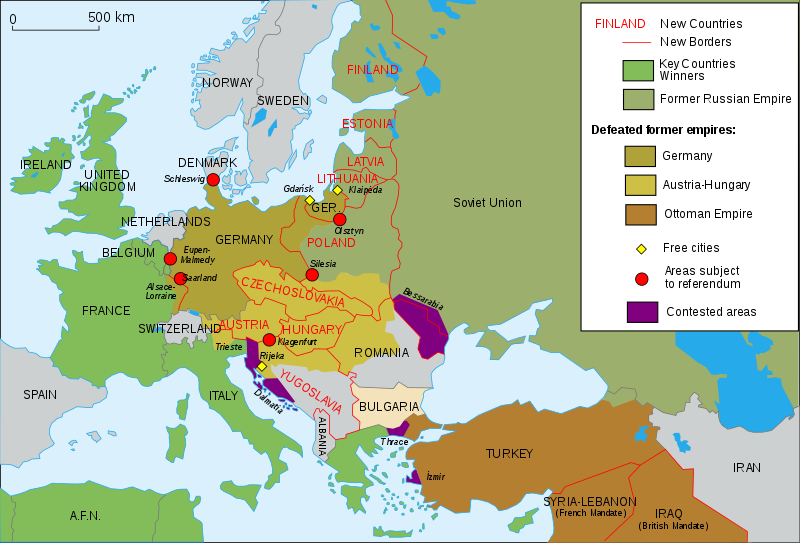
\includegraphics[width=0.8\textwidth,height=\textheight]{figures/map_europe_1923.png}

}

\caption{\href{https://commons.wikimedia.org/wiki/File:Map_Europe_1923-en.svg}{第1次世界大戦によるヨーロッパにおける国境変更}}

\end{figure}

世界恐慌 (1929年)\(\leadsto\)国際協調は衰退、経済的・軍事的競争の激化

\(\leadsto\)ドイツ、イタリア、日本などのファシスト国家が既存の秩序に挑戦

\hypertarget{ux51b7ux6226ux671f}{%
\subsection{冷戦期}\label{ux51b7ux6226ux671f}}

全く異なるイデオロギーの2つの国が超大国の存在

\begin{itemize}
\tightlist
\item
  アメリカ:資本主義
\item
  ソビエト連邦:共産主義
\end{itemize}

\(\leadsto\)それぞれがブロックを形成、\textbf{国際連合}を中心とする普遍的な協調は困難

\begin{itemize}
\tightlist
\item
  \textbf{NATO}などのアメリカの同盟網と\textbf{ブレトンウッズ体制}
\item
  \textbf{ワルシャワ条約機構}と\textbf{コメコン}
\end{itemize}

\begin{figure}[htpb]

{\centering \includegraphics[width=0.8\textwidth,height=\textheight]{international_history_files/mediabag/Cold_War_Map_1980.png}

}

\caption{\href{https://commons.wikimedia.org/wiki/File:Cold_War_Map_1980.png}{1980年の東西陣営}}

\end{figure}

\textbf{超大国間の戦争がなかった}という意味において、冷戦期は平和な時代

\begin{itemize}
\tightlist
\item
  ベルリン危機(1949年)
\item
  キューバ危機(1962年)
\end{itemize}

ただし、どちらも自らの勢力圏の維持のための他国に介入(\textbf{代理戦争}の場合も)

\begin{itemize}
\tightlist
\item
  アメリカによるベトナム戦争(1955-75年)
\item
  ソ連によるアフガン侵攻(1978-89年)
\end{itemize}

全てが平和的ではなかったが、1960年代半ばまでにほとんどの\textbf{植民地}が独立

\begin{enumerate}
\def\labelenumi{\arabic{enumi}.}
\tightlist
\item
  WWI後(特に世界恐慌後)、植民地が経済的に自立\(\leadsto\)ナショナリズム
\item
  WWII後、宗主国は植民地経営が困難
\item
  アメリカは市場へのアクセスと社会主義化の恐れ\(\leadsto\)植民地独立を支持
\end{enumerate}

\(\leadsto\)本来の意味での主権国家体系が成立

\begin{figure}[htpb]

{\centering 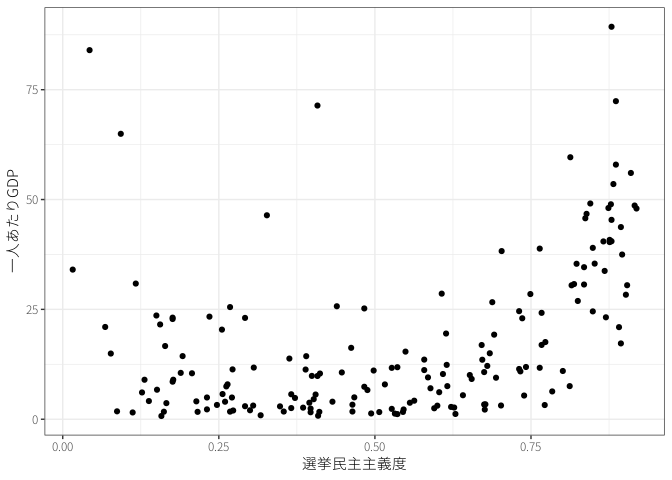
\includegraphics{international_history_files/figure-pdf/unnamed-chunk-2-1.png}

}

\caption{\href{https://correlatesofwar.org/data-sets/state-system-membership/}{国家の数の推移}}

\end{figure}

\begin{figure}[htpb]

{\centering 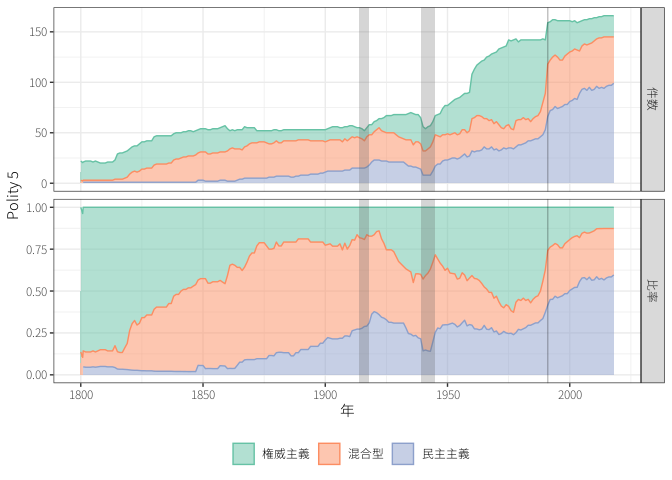
\includegraphics{international_history_files/figure-pdf/unnamed-chunk-3-1.png}

}

\caption{\href{https://correlatesofwar.org/data-sets/state-system-membership/}{各国の独立年}}

\end{figure}

\textbf{南北問題}:経済的に発展している北半球と、そうではない南半球の間の格差問題

\begin{itemize}
\tightlist
\item
  \textbf{非同盟諸国運動} (Non-Aligned Movement: NAM)
\item
  第1次\textbf{石油危機}(1973年)
\end{itemize}

先進国の不況\(\leadsto\) 1980年代の新興国の債務危機

\hypertarget{ux30ddux30b9ux30c8ux51b7ux6226ux671f}{%
\subsection{ポスト冷戦期}\label{ux30ddux30b9ux30c8ux51b7ux6226ux671f}}

冷戦の終結\(\leadsto\)政治的対立が終わり、グローバル化の進展と共に国際協調が促進されると期待

\begin{itemize}
\tightlist
\item
  先進国の経済統合(e.g.,
  \textbf{欧州連合}、\textbf{NAFTA})が深化、新興国や旧東側諸国も自由経済を採用
\item
  \textbf{湾岸戦争}(1990年)において国連が機能、内戦に積極的に介入
\end{itemize}

しかし、2000年以降の国際社会は当初の楽観的な見通しを否定しつつある。

\begin{itemize}
\tightlist
\item
  中東におけるテロ(cf.~\textbf{9.11同時多発テロ})やイスラム国の台頭、民主化(\textbf{アラブの春})と内戦、イランによる核開発
\item
  東アジアにおける\textbf{中国}の経済的・軍事的台頭と領土紛争、北朝鮮による核開発
\item
  ウクライナにおける親欧米政権の成立とロシアによるクリミア併合、東部での軍事衝突、\textbf{ロシア・ウクライナ戦争}の勃発(2022年)
\item
  アメリカの\textbf{単独行動主義} (unilateralism)
  や国際的関与の低下、\textbf{米中対立}
\item
  \textbf{リーマンショック}(2008年)や\textbf{COVID-19}(2020年)に象徴される\textbf{反グローバル主義}やイギリスによるEU脱退などの\textbf{欧州懐疑主義}
  (Euroscepticism)
\end{itemize}

\hypertarget{ux81eaux751fux7684ux306aux79e9ux5e8f}{%
\section{自生的な秩序}\label{ux81eaux751fux7684ux306aux79e9ux5e8f}}

平和や安定を維持するために選択された主権国家体系

\begin{itemize}
\tightlist
\item
  国家の誕生:権力・暴力を独占させることで、国内秩序を維持する。
\item
  主権国家体系の誕生:内政不干渉によって、国際秩序を維持する。
\end{itemize}

国際関係は安定的・協調的ではないが、対立で満ちた無秩序でもない。

\begin{itemize}
\tightlist
\item
  notホッブズのいう「万人の万人に対する闘争」
\end{itemize}

\begin{figure}[htpb]

{\centering \includegraphics[width=0.8\textwidth,height=\textheight]{figures/gdp-per-capita-maddison-2020.png}

}

\caption{一人あたりGDPの長期的変化}

\end{figure}

\begin{figure}[htpb]

{\centering \includegraphics[width=0.8\textwidth,height=\textheight]{figures/population.png}

}

\caption{人口の長期的変化}

\end{figure}

\(\leadsto\)アナーキーな社会において、(中央)\textbf{政府なき統治}
(governance without government) を(部分的に)実現している。

\begin{itemize}
\tightlist
\item
  国家の自発的な行動によって形成される\textbf{自生的}・自己拘束的
  (self-enforcing) な秩序
\end{itemize}

\begin{enumerate}
\def\labelenumi{\arabic{enumi}.}
\tightlist
\item
  なぜ、中央集権的政治体の存在しない分権的社会で、協調が可能なのか?

  \begin{itemize}
  \tightlist
  \item
    アナーキー\(\neq\)対立、中央政府\(\neq\)安定
  \end{itemize}
\item
  なぜ、時代や地域、国際問題によって、国際関係は協調的であるか対立的であるのかが変わるのか?

  \begin{itemize}
  \tightlist
  \item
    人間の本性やアナーキーだけで国際関係の性質を説明するのは難しいようである。
  \end{itemize}
\end{enumerate}

\(\leadsto\)本当に国際的なルール(条約や決議)は無意味?

\begin{itemize}
\tightlist
\item
  無意味ならば、わざわざ決議の投票行動を重視したり、条約の締結に時間や労力をかけたり、国際裁判に欠席したりしないのでは?
\end{itemize}

\(\leadsto\)様々な問題領域において、国家はどのように自生的秩序を形成し、維持しているのか、その限界はなにかを学ぶ。


  \bibliography{references.bib}


\end{document}
